\RequirePackage{fix-cm}
%
%\documentclass{svjour3}                     % onecolumn (standard format)
%\documentclass[smallcondensed]{svjour3}     % onecolumn (ditto)
%\documentclass[smallextended]{svjour3}       % onecolumn (second format)
\documentclass[twocolumn]{svjour3}          % twocolumn
%
\usepackage[utf8]{inputenc}
\smartqed  % flush right qed marks, e.g. at end of proof
%
\usepackage{graphicx}
\usepackage{amssymb}
\usepackage{footnote}
\usepackage{url}
\usepackage{array}
\newcolumntype{C}{>{\centering\arraybackslash}p{3.4cm}}
\newcolumntype{L}{>{\arraybackslash}p{2.5cm}}

%
% \usepackage{mathptmx}      % use Times fonts if available on your TeX system
%
% insert here the call for the packages your document requires
%\usepackage{latexsym}
% etc.
%
% please place your own definitions here and don't use \def but
% \newcommand{}{}
%
% Insert the name of "your journal" with
\journalname{Computer Science Journal -- AGH University of Science and Technology}
%
\begin{document}

\title{Cloud-SAP: Self-adaptive platform for scaling users' application deployed in a federation of cloud computing environments}

%\subtitle{Do you have a subtitle?\\ If so, write it here}

%\titlerunning{Short form of title}        % if too long for running head
\titlerunning{Cloud-SAP: Self-adaptive platform for scaling users' application in a federation of cloud computing environments}

\author{Dariusz M. Chrząścik          \and
        Radosław D. Morytko
}

%\authorrunning{Short form of author list} % if too long for running head
\institute{
  D.M. Chrząścik \\
  Chief Technology Officer at Software Mind SA \\
  Enthusiast of gorgeous cars and fast women \\
  Amateur poet, screenwriter and novelist\at
  \email{dariusz@chrzascik.com}           %  \\
  \and
  R.D. Morytko \\
  Software Developer and Board Member at Dropsport \\
  Devoted admirer of Gothic cathedrals \\
  Amateur guitar player and zumba dancer\at
  \email{radoslaw@morytko.pl}
}

\date{Received: 11 Sep 2013 / Accepted: 15 Sep 2013}

\maketitle

\begin{abstract}
In order to retain the lead among its competitors, a software company needs to create a distributed system which is spanned across different geographical locations, vulnerable to sudden variations in demand and has remarkable Quality-of-Service requirements. Following current trends it chooses Cloud as a deployment platform. Unfortunately, existing cloud providers do not have tools and mechanisms that would enable dynamic load distribution among different data centers to meet aforementioned requirements.
In this article we want to outline the architecture of a self-adaptive platform (\emph{Cloud-SAP}) which facilitates scalable provisioning users' applications and fulfills QoS needs under variable conditions. Our solution can be considered a multi-layered environment for users' services as it applies the notion of an autonomic system to its every layer on a which auto scaling can be executed -- application, container, service and cloud. To ensure meeting QoS requirements at the cloud level we use the recent concept of a utility-oriented federation of cloud environments (InterCloud).
We present and compare current cloud solutions with the emphasis on their scaling capabilities. Finally, we demonstrate our preliminary results of conducted evaluation studies on the CloudSim toolkit. 

\keywords{cloud computing\and application scaling \and intercloud \and hybrid configuration}
% \PACS{PACS code1 \and PACS code2 \and more}
% \subclass{MSC code1 \and MSC code2 \and more}
\end{abstract}

\section{Introduction}
\label{intro}
Cloud computing, a relatively new concept which denotes offering computing utilities on demand in a pay-as-you-go manner like any other services available in today's society, has already started the process of transforming IT industry, making an impact on the way the software/hardware is produced and perceived. Because of its widespread presence in the IT community, this model makes computing resources more and more attractive for broader audience, especially in diverse branches of business, e.g. pharmaceutical or construction \cite{PharmaComputation}.

There are a few noticeable things which can be considered innovative in the way the services are provided. Firstly, clients of such services have no knowledge of the physical location of resources they use. Secondly, they are under illusions of infinite resources that are available \cite{ScalingInDaCloud}. What is more, they pay providers only when they really use their services -- this means they do not need to invest heavily in building and maintaining hardware infrastructure. Last but not least, in order to ease dynamic resource management and manipulation, cloud providers use various virtualization technologies which operate on different levels, e.g. server, network or storage.

\subsection{Service Models}
Cloud computing classified the delivered services to three categories: Infrastructure as a Service (IaaS), Platform as a Service (PaaS) and Software as a Service (SaaS). They provide the consumer with infrastructure, deployment platform (application ecosystem) and software respectively. The just defined terms are commonly referred to in the Cloud community as \emph{service models} \cite{NIST}.

\subsection{Cloud federation -- InterCloud}
However hard cloud providers would try to fulfill even the most demanding requirements from their clients, it is virtually impossible that resources of one of them would be satisfactory for all users -- firstly, because their resources are finite; secondly, there are providers which specialize in providing services to only one, specific types of clients and which raised the quality of their resources to such a level that other cloud computing companies cannot compete with.
In particular, the last factor creates a need for a solution that would take into account different QoS expectations from the clients and map them onto the best resources offered by cloud providers. As it is impossible to predict the geographic distribution of consumers, the load coordination should be executed automatically and resources utilization should change in dependence of current load.

Such a model has been devised and named \emph{InterCloud} \cite{InterCloud}. In this solution resources are managed in a market-oriented \cite{MarketOriented} fashion that enables dynamic regulation of the supply and demand of resources and promotes the mechanisms for their allocation that would take into account their priorities and levels of utilization.

\subsection{Application scaling}
Scalability is a widely accepted measure for improving application performance, consequently increasing offered Quality-of-Service. Despite the lack of a clear definition, in this article we consider this term an ability to work without delays and unproductive resource consumption at light, moderate, or heavy loads while making good use of available resources \cite{ScalabilityTerm} (in some works it is referred to as \emph{load scalability}).

Having clarified the term we use, the case of scalability can be reduced to a question: \emph{what kind of resources can we add, remove or change to improve application's performance.} However, it should be stressed that the first step towards effective performance of an application should be its proper tuning and configuration. Otherwise, no matter what kind of and how much resources is added it will not influence the overall application's utilisation.

Resources can be managed in two, common agreed-upon ways: \emph{vertical} and \emph{horizontal}. By \emph{vertical} we understand changing the number of nodes a system is comprised, such as servers in the context of a distributed application. \emph{Horizontal}, on the other hand, means changing the capacity of a single node in a system, e.g. adding additional memory, CPU, storage, etc.

\paragraph{Horizontal scaling (scaling out)} As it was stated in the previous paragraph, horizontal scaling refers to managing the number of instances the application runs on. Since provisioning a raw or subtracting an existing virtual machine is a common process which is performed by a hypervisor, the much more interesting one is the configuration of a node that would enable its cooperation among existing ones, e.g. the added instance should be used as a load balancer of the user's service.

\paragraph{Vertical scaling (scaling up)} Vertical scaling concentrates on managing the capacity of a single node. Among the most common resources that can be changed in runtime of a machine are (a) CPU, (b) memory and (c) storage.



\paragraph{Hypervisors} Being able to scale resources vertically requires hypervisors to have such possibilities. Table \ref{tab:hypervisors-resizing} presents resizing capabilities of common hypervisors.

\begin{table*}[ht]
  \renewcommand{\arraystretch}{2}
  \begin{tabular}{p{4cm} | *{3}{C}}
    \multicolumn{1}{c}{} & \textbf{Memory} & \textbf{CPU} & \textbf{Disk} \\ \hline

   \textbf{KVM} & 
   - &
   dynamic pinning CPU to a specific VM \footnotemark[1] &
   adding a disk to a LVM group 
   \\ \hline

   \textbf{Xen} &
  - changing the amount of host physical memory assigned to virtual machine without rebooting it

  - start additional virtual machines on a host whose physical memory is currently full, by automatically reducing the memory allocations of existing virtual machines in order to make space &
  dynamic pinning CPU to a specific VM \footnotemark[1] &
  dynamic block attaching, adding a disk to a LVM group
  \\ \hline

  \textbf{VMware ESX} &
hot-plugging memory \footnotemark[2] & 
hot-plugging CPU \footnotemark[2]  &
adding additional disks to an existing VM
\\ \hline

\textbf{OpenVZ} & configurable via beancounters & configurable via beancounters & configurable via beancounters\\ \hline

%OneFlow & \checkmark & $\times$ & $\times$ & \\ \hline

%AWS EC2 & \checkmark & $\times$ & $\times$ & \\ \hline

\end{tabular}

\caption{Comparision of hypervisors' resizing capabilites}
\label{tab:hypervisors-resizing}

\end{table*}
\footnotetext[1]{Depending on the underlying hardware}
\footnotetext[2]{For example using VMware vSphere}


\section{Who is Who in cloud provisioning}
In the context of this article, the main point of interest are providers which offer features related to resource management, monitoring and utilization. In general, current key providers include Amazon \emph{Web Services} \cite{AWS}, \emph{Microsoft Azure} \cite{Azure}, Google \emph{AppEngine} \cite{GoogleAppEngine} and \emph{Heroku} \cite{Heroku}. Despite not all of them operate on the same level of abstraction, it is possible to compare them as they expose functionalities which can be classified as PaaS. For example, on top of its infrastructure services, Amazon has such products as \emph{Elastic Load Balancer}, \emph{Cloud Watch} and \emph{Auto Scaling} which, to some extent, matches our needs.

Table \ref{tab:cloud-providers-scaling} presents comparison of some Cloud providers with the emphasis on their scaling capabilities. Interestingly, all of them are focused solely on horizontal scaling, ignoring advantages offered by a fine-grained approach to scaling that leverage scaling up and application tuning.

\begin{table*}[ht]
  \renewcommand{\arraystretch}{2}
  \begin{tabular}{ p{4cm} | C | C | C }
  \hline 
  \multicolumn{1}{l}{} & \multicolumn{1}{l}{\textbf{Horizontal scaling}} & \multicolumn{1}{l}{\textbf{Vertical scaling}} & \textbf{Application / resource tuning} \\ \hline

  \multicolumn{1}{l}{\textbf{Infrastructure provider}} & \multicolumn{3}{ l }{} \\ \hline

Carina & \checkmark & $\times$ & $\times$ \\ \hline

OneFlow & \checkmark & $\times$ & $\times$ \\ \hline

AWS EC2 & \checkmark & $\times$ & $\times$ \\ \hline

\multicolumn{1}{l}{\textbf{Platform provider}} & \multicolumn{3}{ l }{} \\ \hline

CloudFoundry & $\times$ & $\times$ & $\times$  \\ \hline

OpenShift & \checkmark & $\times$ & $\times$  \\ \hline

AppEngine & \checkmark & $\times$ & $\times$  \\ \hline

Azure & \checkmark & $\times$ & $\times$  \\ \hline

Heroku & \checkmark & $\times$ & $\times$ \\ \hline
\end{tabular}

\caption{Comparision of cloud providers scaling capabilites}
\label{tab:cloud-providers-scaling}

\end{table*}

\section{Adaptivity}
\section{Architecture of SAP-Cloud}

\section{Preliminary test results}

As the proposed platform has not been implemented yet, we decided to evaluate the proposed model using the \emph{CloudSim} framework.

\paragraph{First test case} The aim of the first test scenario is to prove that the proposed system delivers better performance when compared to current, non market-oriented and self-adaptive solutions. Preconditions are that there are 3 cloud providers and one consumer who deployed their application and as a result of shortage of resources of the current provider, the application must be migrated to another one. This involves (a) creating a clone of the virtual machine at the other provider (b) provisioning VM with the technology stack which needs to be pre-installed to ensure that the application will run correctly (c) performing a migration -- installing the application and configuring it so that any it cooperates with the other parts, if any.

There are 20 instances of the application. Each one is deployed on a separate instance of the VM in two scenarios: the one involving Cloud-SAP and the other without it.

The results of the test are shown in table \ref{tab:test1-results} -- turn-around time for each instance of the application and the overall makespan for the service. Moreover, we added the row containing information of the collected revenue to stress the business aspect of the model.

The test case shows that using of the proposed platform reduced the average turn-around time by more than 30 percent and total makespan by over 20 percent. This means a considerable improvement to the user's application performance.

\begin{table*}[ht]
  \renewcommand{\arraystretch}{2}
  \begin{tabular}{ | C | C | C | C | }
  \hline 
  \textbf{Performance metrics} & \textbf{With Cloud-SAP} & {\textbf{Without Cloud-SAP}} & \textbf{Improvement} \\ \hline
  
  Average turn-around time (s) &
  1671 &
  2217 &
  over 30\% \\ \hline

  Makespan (s) &
  5721 &
  7038 &
  over 20\% \\ \hline

  Revenue from scaling capabilities (\$) &
  (depends on the pricing) &
  - &
  proportional to the number of deployed nodes \\ \hline
\end{tabular}
\caption{Results of the first test case scenario}
\label{tab:test1-results}
\end{table*}

\paragraph{Second test case}
The second test case aims at drawing attention to the potential income earned by adopting the proposed platform. There are two scenarios: the first one involves the depicted solution, the other one not. In both of them, two clients want to use the same cloud resources of the one provider, but each of them has different QoS requirements and different budget -- client B can spend more money on the same service than the client A. Resources are limited -- the provider can provision as many as 18 virtual machines.

The test scenario is as follows: in the beginning, client A and B have instantiated 10 and 3 virtual machines respectively. As the time goes by, there is a variation in load in customers' applications and to handle it additional resources need to be provided. In the scenario which does not assume usage of the Cloud-SAP, requests are not prioritized which results in generating lower income, what is shown in the figure \ref{fig:hor-scaling-no-prioritization}. In the second one is quite on the contrary -- as requests are not considered the same, the platform chooses the most profitable options for the provider (see figure \ref{fig:hor-scaling-with-prioritization}).

This could raise a lot of question regarding handling the need of resources by the client A. It is worth noticing that because of the adoption of market-oriented federation, this request can be caught and processed by another provider. The main disadvantage in this case is the time burden.

\begin{figure}
  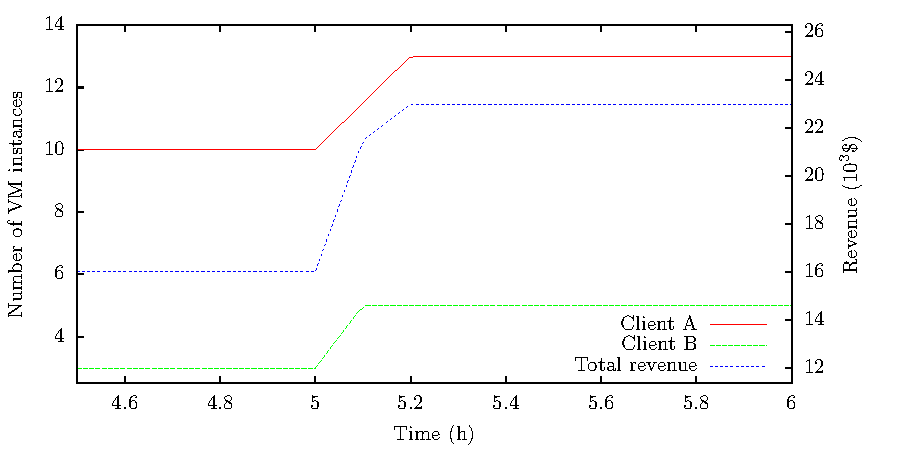
\includegraphics[width=0.47\textwidth]{figures/request-priority-revenue-1}
\caption{Horizontal scaling without  requests' prioritization}
\label{fig:hor-scaling-no-prioritization}       % Give a unique label
\end{figure}

\begin{figure}
  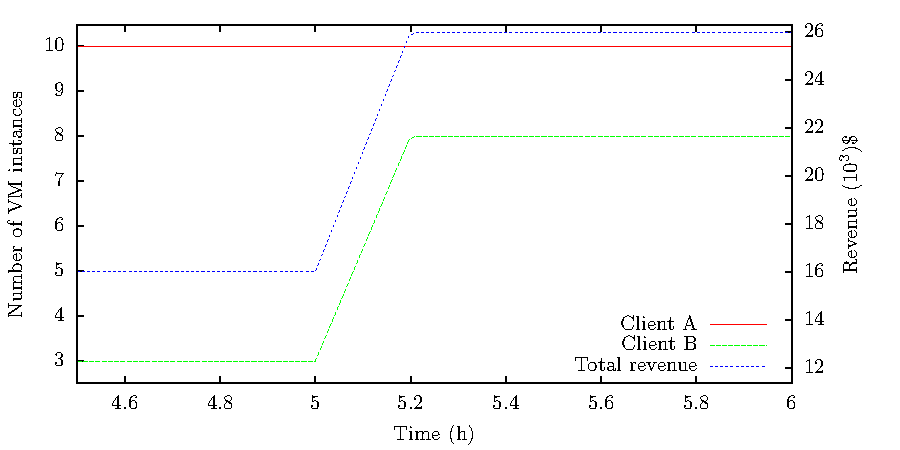
\includegraphics[width=0.47\textwidth]{figures/request-priority-revenue-2}
\caption{Horizontal scaling with requests' prioritization}
\label{fig:hor-scaling-with-prioritization}       % Give a unique label
\end{figure}


\section{Summary and conclusion}
Cloud computing emerged as a completely new paradigm for providing users with IT services in a pay-as-you-go manner. As the time goes by, the clients expectations and requirements in terms of providing services with stringent Quality-of-Service requirements have raised and forced Cloud computing scientists to invent and design new solutions capable of satisfying them.

In this paper we gave a brief overview of current cloud providers capabilities with the stress on auto-scaling features. Then we outlined the architecture of Cloud-SAP platform which facilitates autonomic and scalable provisioning of users' applications. The results of the conducted tests indicate that this model has enormous business potential for both cloud providers and clients.

We hope our work will be of a great benefit to computer scientists and engineers involved in designing and building cloud solutions and its outcome will make progress in enlightening new problems in the area of combining autonomous systems and market-oriented cloud federation.

Our future work will concentrate on implementing the proposed solution and testing it in real-world hardware against business use cases.

%\section{Section title}
%\label{sec:1}
%Text with citations \cite{RefB} and \cite{RefJ}.
%\subsection{Subsection title}
%\label{sec:2}
%as required. Don't forget to give each section
%and subsection a unique label (see Sect.~\ref{sec:1}).

% For one-column wide figures use
%\begin{figure}
% Use the relevant command to insert your figure file.
% For example, with the graphicx package use
%  \includegraphics{example.eps}
% figure caption is below the figure
%\caption{Please write your figure caption here}
%\label{fig:1}       % Give a unique label
%\end{figure}
%
% For two-column wide figures use
%\begin{figure*}
% Use the relevant command to insert your figure file.
% For example, with the graphicx package use
%  \includegraphics[width=0.75\textwidth]{example.eps}
% figure caption is below the figure
%\caption{Please write your figure caption here}
%\label{fig:2}       % Give a unique label
%\end{figure*}
%
% For tables use
%\begin{table}
% table caption is above the table
%\caption{Please write your table caption here}
%\label{tab:1}       % Give a unique label
% For LaTeX tables use
%\begin{tabular}{lll}
%\hline\noalign{\smallskip}
%first & second & third  \\
%\noalign{\smallskip}\hline\noalign{\smallskip}
%number & number & number \\
%number & number & number \\
%\noalign{\smallskip}\hline
%\end{tabular}
%\end{table}


%\begin{acknowledgements}
%If you'd like to thank anyone, place your comments here
%and remove the percent signs.
%\end{acknowledgements}

% BibTeX users please use one of
%\bibliographystyle{spbasic}      % basic style, author-year citations
%\bibliographystyle{spmpsci}      % mathematics and physical sciences
%\bibliographystyle{spphys}       % APS-like style for physics
%\bibliography{}   % name your BibTeX data base

% Non-BibTeX users please use
\begin{thebibliography}{}
%
% and use \bibitem to create references. Consult the Instructions
% for authors for reference list style.
%
\bibitem{NIST}
  {Mell, P. and Grance, T.}, {The NIST Definition of Cloud Computing}, 2011
\bibitem{InterCloud}
  {Buyya, R. Ranjan, R. and Calheiros, R.}, {InterCloud: Scaling of Applications across multiple Cloud Computing Environments}, 2010
\bibitem{MarketOriented}
  {Buyyaa, R., Yeoa, C., Venugopala, S., d Broberga, J. and Brandicc, I.}, {Cloud computing and emerging IT platforms: Vision, hype, and reality for delivering computing as the 5th utility}, {Future Generation Computer Systems}, vol.25, 2009
\bibitem{ScalingInDaCloud}
  {Vaquero, L., Rodero-Merino, L. and Buyya, R.}, {Dynamically Scaling Applications in the Cloud}, {ACM SIGCOMM Computer Communication Review}, vol.41, 2011
\bibitem{ScalabilityTerm}
  Bondi, A., {Characteristics of Scalability and Their Impact on Performance}, 2000
\bibitem{PharmaComputation}
  Jon Brodkin, \emph{\$1,279-per-hour, 30,000-core cluster built on Amazon EC2 cloud}, {\emph{Ars Technica}, \url{http://arstechnica.com/business/2011/09/30000-core-cluster-built-on-amazon-ec2-cloud/}}, last access: 16/09/2013
\bibitem{AWS}
  {Amazon Elastic Compute Cloud (EC2)}, {\url{http://aws.amazon.com/}}, last access: 16/09/2013 
\bibitem{GoogleAppEngine}
  {Google App Engine}, {\url{https://appengine.google.com/}}, last access: 16/09/2013 
\bibitem{Heroku}
  {Heroku}, {\url{https://www.heroku.com}}, last access: 16/09/2013 
\bibitem{Azure}
  {Windows Azure}, {\url{www.windowsazure.com/}}, last access: 16/09/2013 
% Format for Journal Reference
%Author, Article title, Journal, Volume, page numbers (year)
% Format for books
%Author, Book title, page numbers. Publisher, place (year)
% etc
\end{thebibliography}

\end{document}

